\section{Parte III}
    \subsection{Gráfico}
        \begin{figure} [H] 
            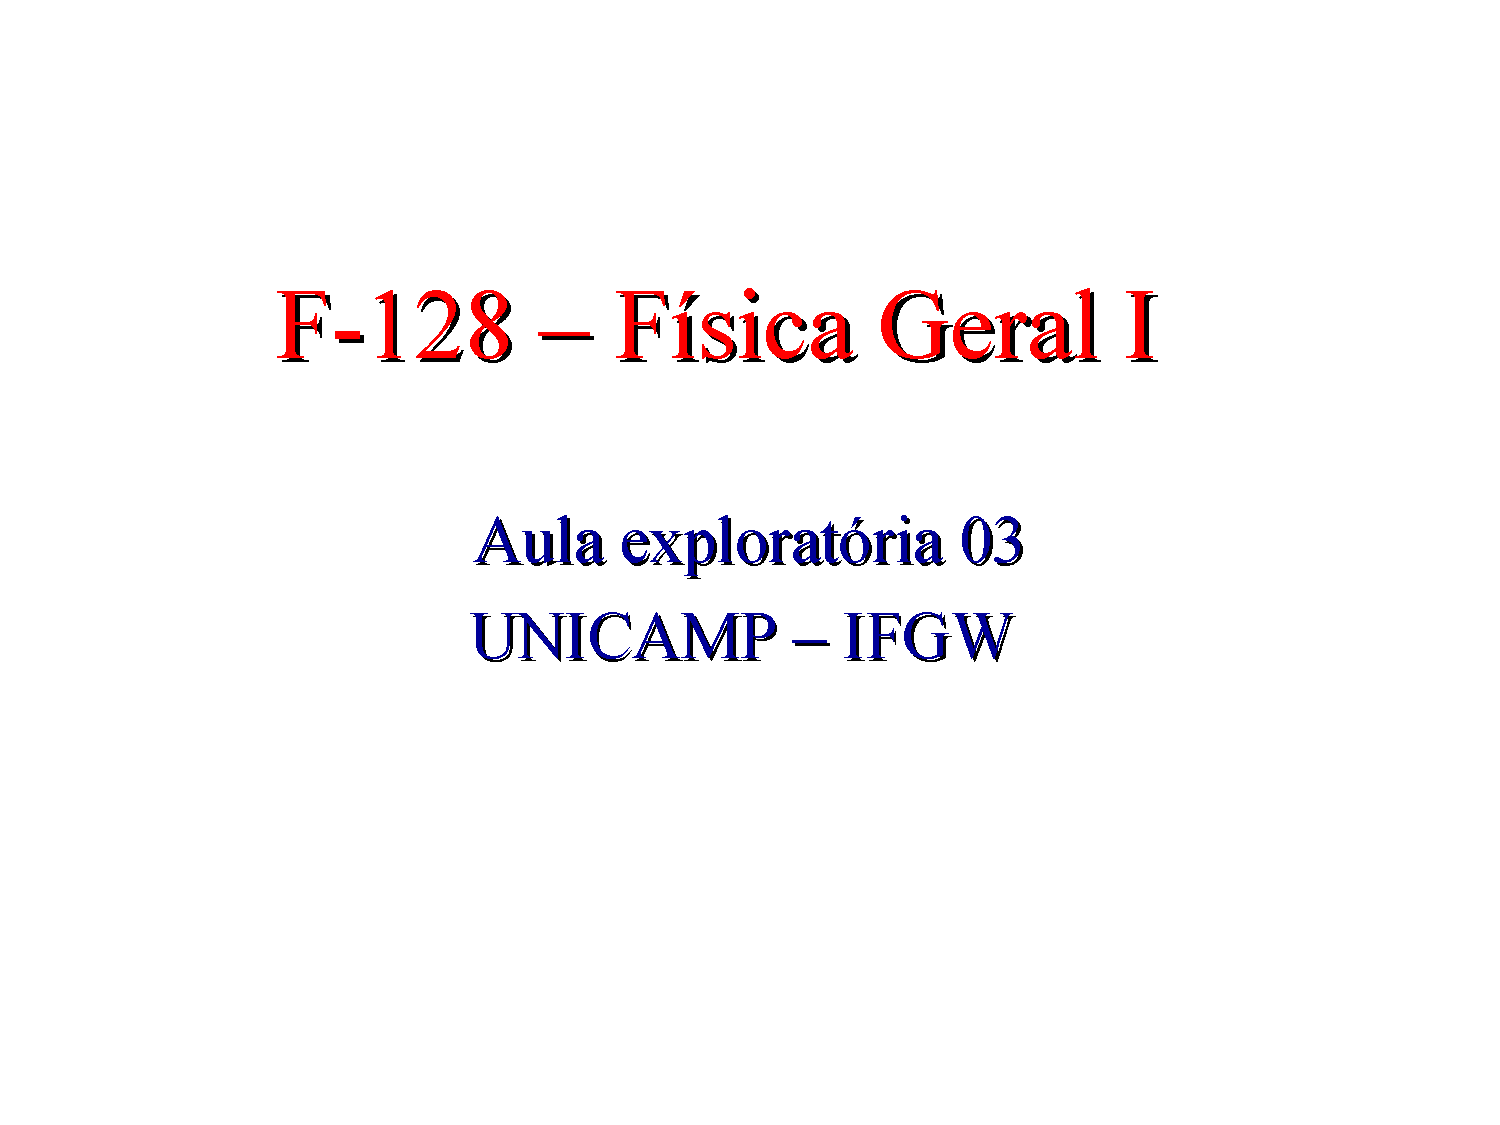
\includegraphics[width=\textwidth]{03}
            \caption{Gráfico de $\tau$ por $\frac{1}{d}$}
            \label{fig:03}
        \end{figure}

    \subsection{Constante dielétrica do papel}
        Sabendo que a constante dielétrica depende apenas da geometria do 
        material e da relação $\tau = RC$ podemos escrever a relação entre $\tau$,
        a resistência do circuito e a geometria do capacitor da segunte forma:

        $$\tau = \epsilon_0 R A \times \frac{1}{d} k$$

        Onde k é a constande dielétrica a ser estudada.
        
        De acordo com os dados obtidos no experimento, obtemos um valor de:

        $$k_{teorico} = \frac{\tau d}{\epsilon_0 R A} = 7,04$$
        $$\Delta k_{teorico} = 
        \sqrt{(\frac{d}{R \epsilon_0 A})^2 \Delta\tau^2 + 
        (\frac{\tau}{R \epsilon_0 A})^2 \Delta d^2 + 
        (\frac{\tau d}{R^2 \epsilon_0 A})^2 \Delta R^2 + 
        (\frac{\tau d}{R \epsilon_0 A^2})^2 \Delta A^2} = 0.04$$

        Logo:

        $$k_{teorico} = 7,04 \pm 0,04$$

        E praticamente pelo coeficiente angular:

        $$a = 9,439\times10^{-9}$$
        $$\Delta a = 3\times10^{-33}$$

        Usando:

        $$a = k\epsilon_0 R A 
        \Rightarrow k = \frac{a}{\epsilon_0 R A}$$
        $$\Delta a = \sqrt{
            (\frac{1}{\epsilon_0 R A})^2 \Delta a^2 +
            (\frac{a}{\epsilon_0 R^2 A})^2 \Delta R^2 +
            (\frac{a}{\epsilon_0 R A^2})^2 \Delta A^2
        }$$

        Logo:

        $$k = (6 \pm 1)$$

    \subsection{Valores obtidos vs Valor esperado}

        O valor da constante dielétrica do papel esperada 
        estava entre 4 e 6, porém o encontrado
        teoriacamente foi $7,04 \pm 0,04$ o 
        que não condiz, mas experimentalmente
        $6 \pm 1$ está dentro do esperado.

        A constante dielétrica provavelmente se encontrou
        mais alta que o esperado pelo papel utilizado ser
        reciclado, por ter ar entre o papel e por ter sido
        desconsiderado a área do furo dos círculos de papel.
    \subsection{Capacitância `parasita`} 

        A partir do coeficiente linear do gráfico linearizado:

        $$b = 1,657\times10^{-6}$$
        $$\Delta b = 3\times10^{-7}$$

        Podemos encontrar a Capacitância \say{parasita} $C_p$

        $$C_p = \frac{b}{R}$$
        $$\Delta C_p = \sqrt{(\frac{1}{R})^2 \Delta b^2 + (-\frac{b}{R^2})^2 \Delta R^2}$$

        Logo:

        $$C_p = 1,686 \times 10^{-10} F = 169 pF$$
        $$\Delta C_p = 4,59\times10^{-11} F = 46 pF$$

        O que se aproxima mas não abranje o alor esperado
        de 96pF (uma vez que o comprimento do cabo
        era de 1m).

    \subsection{Hipótese para calcular capacitância}

            Na analise dos dados obtidos em relação à capacitância pode-se notar que na hipotese utilizada para determinar seu valor, para quando a distancia é muito menor que o diametro, verifica-se que o calculo da constante dielétrica possui maior precisão. 
        Dessa forma, obtem-se também um valor mais preciso para a capacitancia desejada. Assim, a hipótese utilizada mostra-se válida nesse caso. 